\documentclass[11pt,letterpaper]{article}
\usepackage{../assets/scientific_report}
\usepackage[brazil]{babel}
\usepackage{amsmath,float,listings,xcolor,graphicx,geometry}
\geometry{headheight=23pt,top=2cm,bottom=2cm,left=2.5cm,right=2.5cm}
\setlength{\parskip}{0.5em}
\setlength{\parindent}{0pt}
\lstset{language=C,basicstyle=\ttfamily\small,keywordstyle=\color{blue}\bfseries,commentstyle=\color{green!60!black}\itshape,stringstyle=\color{red!80!black},numbers=left,numberstyle=\tiny\color{gray},numbersep=8pt,frame=single,breaklines=true,captionpos=b,tabsize=4,showstringspaces=false}

\begin{document}
\pagestyle{plain}

\begin{center}
{\LARGE\bfseries Escalabilidade com afinidade de threads no NPAD}\\[0.4em]
{\normalsize Eugenio Vitor Lopes dos Santos}\\[0.3em]
{\small DCA3703, Programação Paralela, Universidade Federal do Rio Grande do Norte}
\end{center}

\section{Enunciado}
\begin{quote}
Avaliar como a escalabilidade do código de Navier--Stokes muda com os tipos de afinidade de threads suportados pelo sistema operacional e pelo OpenMP, no mesmo nó de computação do NPAD usado na Tarefa 12.
\end{quote}

\section{Fundamentação}
O experimento usa, sem alterações numéricas, a versão \texttt{v4\_numa.c} da Tarefa 12. O programa calcula a parcela difusiva em uma malha bidimensional com um stencil de cinco pontos e dois campos em \texttt{double}. Executa 500 passos e distribui blocos contíguos de linhas com \texttt{schedule(static)}. A barreira implícita do \texttt{omp for} é necessária porque o passo seguinte lê o campo produzido no passo anterior.

A inicialização paralela escreve os dois campos antes da evolução. Pelo princípio de \textit{first touch}, essa escrita influencia o domínio NUMA associado às páginas. Manter a afinidade entre a inicialização e o stencil favorece o acesso local à memória. A diretiva \texttt{omp simd} atua no laço interno, enquanto duas variáveis de ambiente controlam a afinidade:

\begin{itemize}
\item \texttt{OMP\_PROC\_BIND=false}: o runtime não fixa a afinidade das threads e o sistema operacional pode migrá-las;
\item \texttt{OMP\_PROC\_BIND=close}: threads vizinhas ocupam lugares próximos;
\item \texttt{OMP\_PROC\_BIND=spread}: o runtime distribui as threads entre os lugares disponíveis;
\item \texttt{OMP\_PLACES=cores|threads}: cada lugar representa um núcleo físico ou uma CPU lógica.
\end{itemize}

O experimento comparou quatro configurações: sem binding, \texttt{close+cores}, \texttt{close+threads} e \texttt{spread+threads}. A combinação \texttt{spread+cores} foi medida na Tarefa 12 e não integra os resultados deste relatório.

\section{Experimento}
As quatro configurações foram executadas no nó \texttt{r2n19} do NPAD, com uso exclusivo e um processo. O nó possui dois AMD EPYC 7713, 64 núcleos por soquete, duas CPUs lógicas por núcleo e oito domínios NUMA. Todas as configurações usaram o mesmo conjunto de CPUs permitido pelo Slurm, \texttt{0--63,128--191}, e os mesmos domínios de memória. A Tarefa 12 usou o nó \texttt{r2n04}, de mesma topologia. A mudança de nó não atende à exigência do enunciado; a comparação deste relatório se restringe às quatro configurações executadas em \texttt{r2n19}.

As configurações usaram o mesmo código e o mesmo binário. Apenas \texttt{OMP\_PROC\_BIND} e \texttt{OMP\_PLACES} mudaram. O Anexo A apresenta o programa completo sem a instrumentação do PaScal e mantém a conversão da carga-alvo em tamanho de malha.

O PaScal Analyzer combinou $p=1,2,4,8,16,32,64$ threads com sete cargas-alvo de $262\,144$ a $16\,777\,216$ células internas, dobradas a cada nível. Para uma carga-alvo $W$, a malha quadrada tem lado $N=\operatorname{round}(\sqrt{W})+2$, incluindo as bordas. O arredondamento pode fazer a carga efetiva diferir do alvo. Cada execução usou a condição inicial gaussiana e 500 passos.

Cada configuração teve 49 pontos, com uma execução por ponto e sem estimativa de dispersão. Os mapas usam a região \textit{Whole Program (Region 0)}, que inclui alocação, inicialização e evolução.

\section{Resultados}
O mapa \textit{Scalability} do PaScal Viewer combina crescimento de carga e de recursos. As linhas representam $p=2,4,8,16,32,64$ e as colunas $i2$--$i7$ representam cargas crescentes. Tons azuis indicam regiões relativamente favoráveis na escala normalizada do Viewer; tons vermelhos indicam perda relativa. O mapa não fornece tempo em segundos. Este relatório não quantifica tempos, speedup ou eficiência, nem apresenta análises separadas de escalabilidade forte e fraca.

\begin{figure}[H]\centering
\begin{subfigure}{0.48\textwidth}\centering
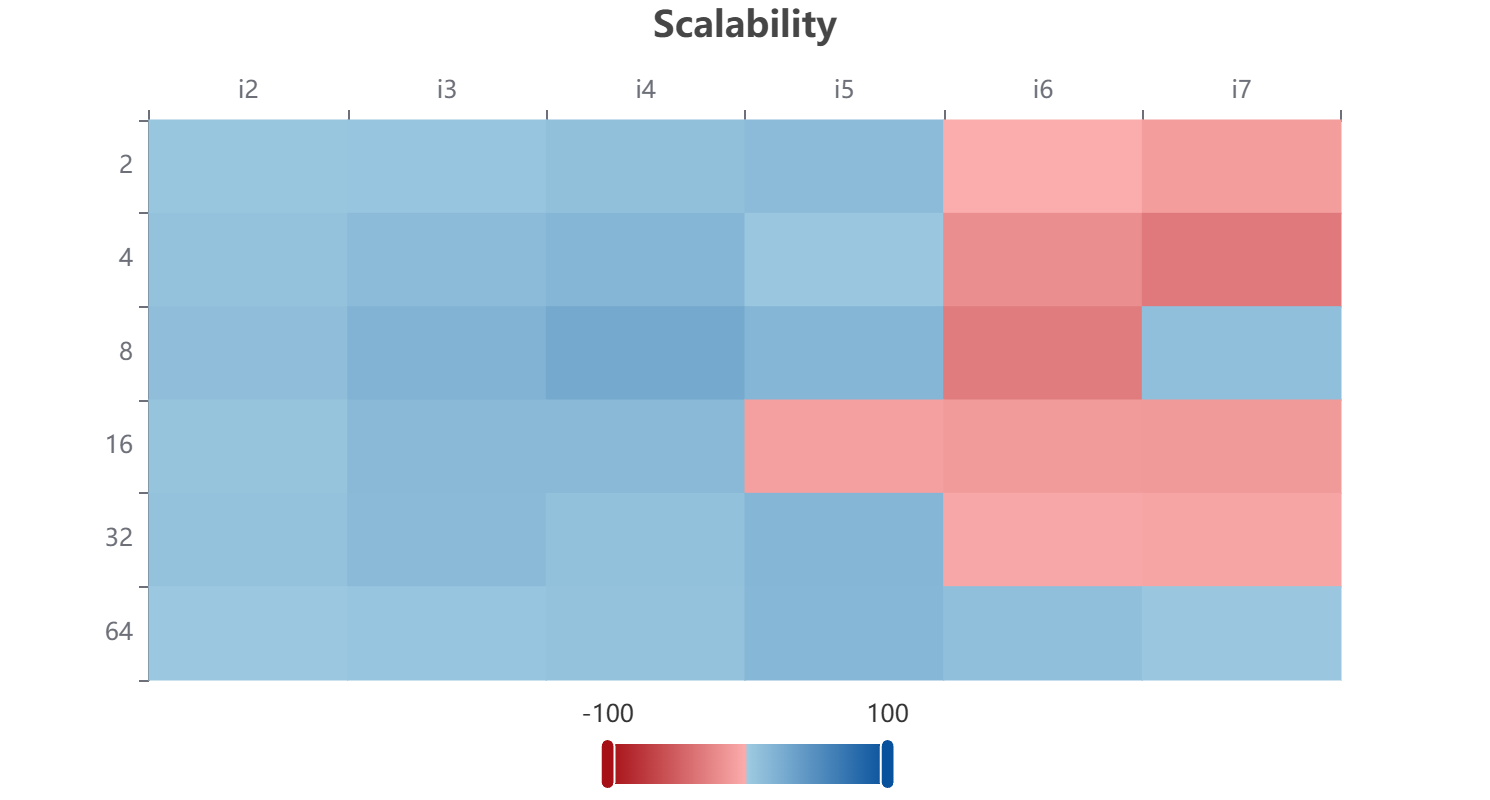
\includegraphics[width=\textwidth]{images/v4_numa_false_Scalability_Whole_Program_(Region_0).png}
\caption{Sem binding OpenMP.}
\end{subfigure}\hfill
\begin{subfigure}{0.48\textwidth}\centering
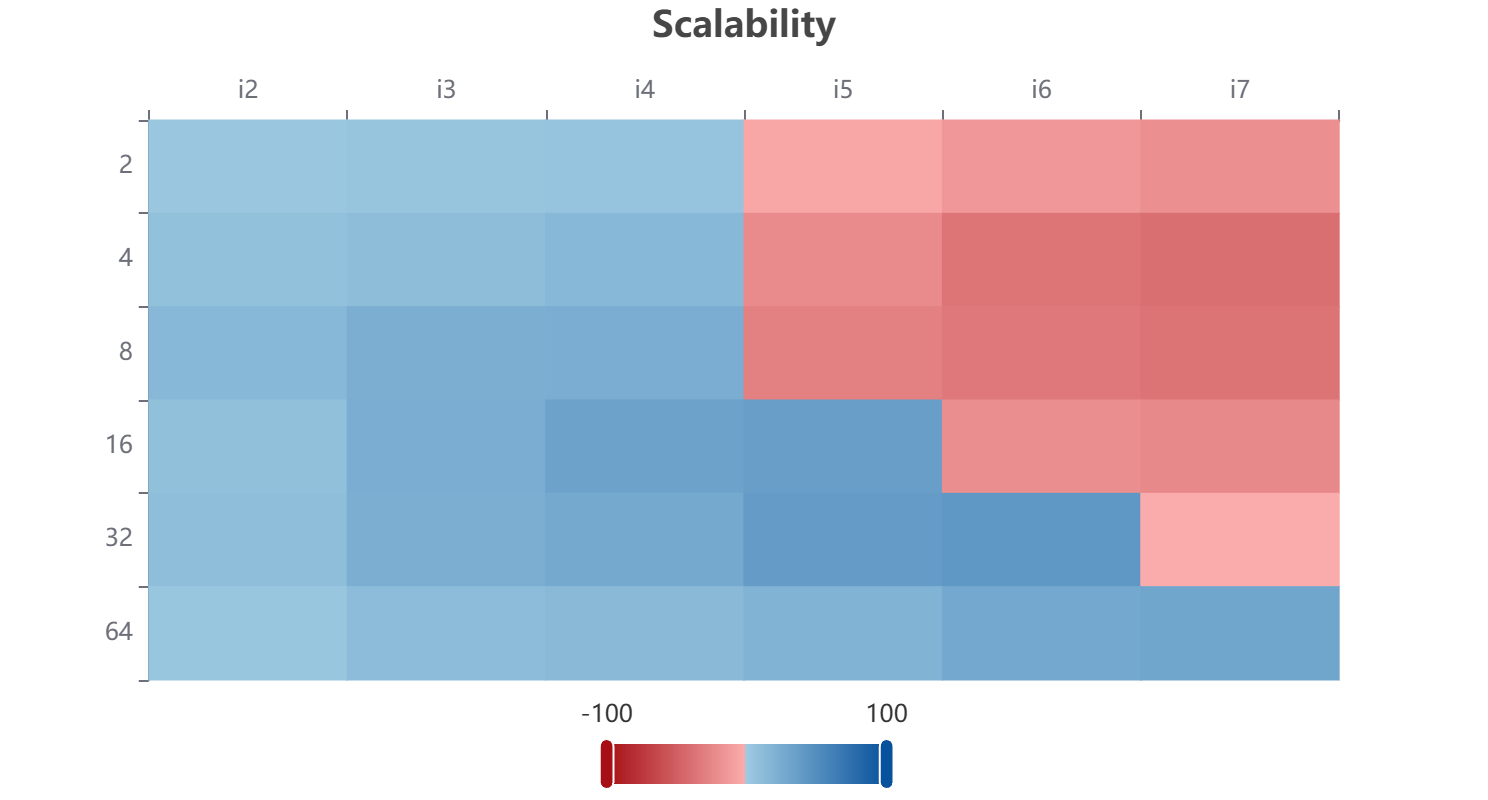
\includegraphics[width=\textwidth]{images/v4_numa_close_cores_Scalability_Whole_Program_(Region_0).png}
\caption{\texttt{close} com lugares por núcleo.}
\end{subfigure}\\[0.7em]
\begin{subfigure}{0.48\textwidth}\centering
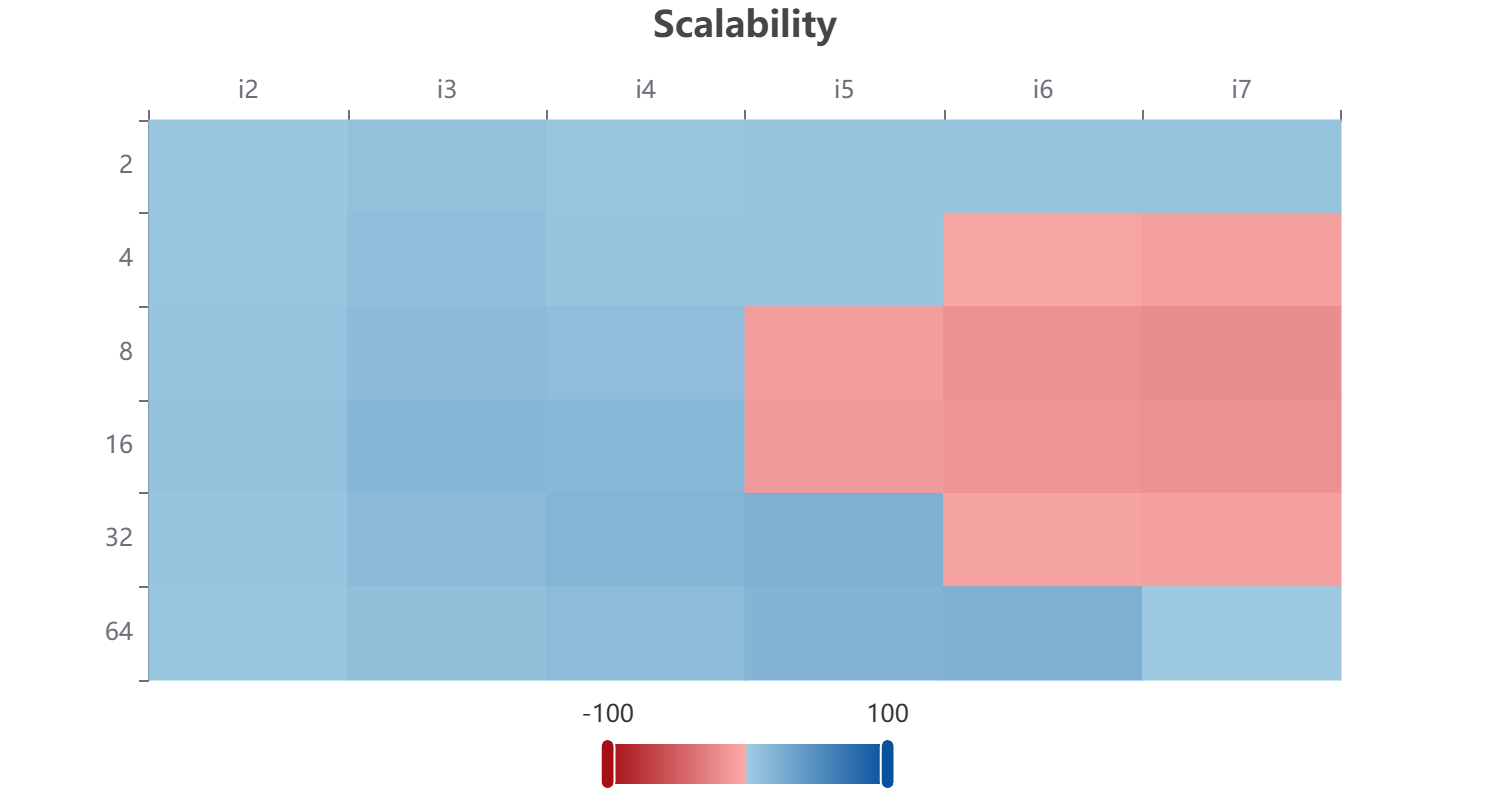
\includegraphics[width=\textwidth]{images/v4_numa_close_threads_Scalability_Whole_Program_(Region_0).png}
\caption{\texttt{close} com lugares por CPU lógica.}
\end{subfigure}\hfill
\begin{subfigure}{0.48\textwidth}\centering
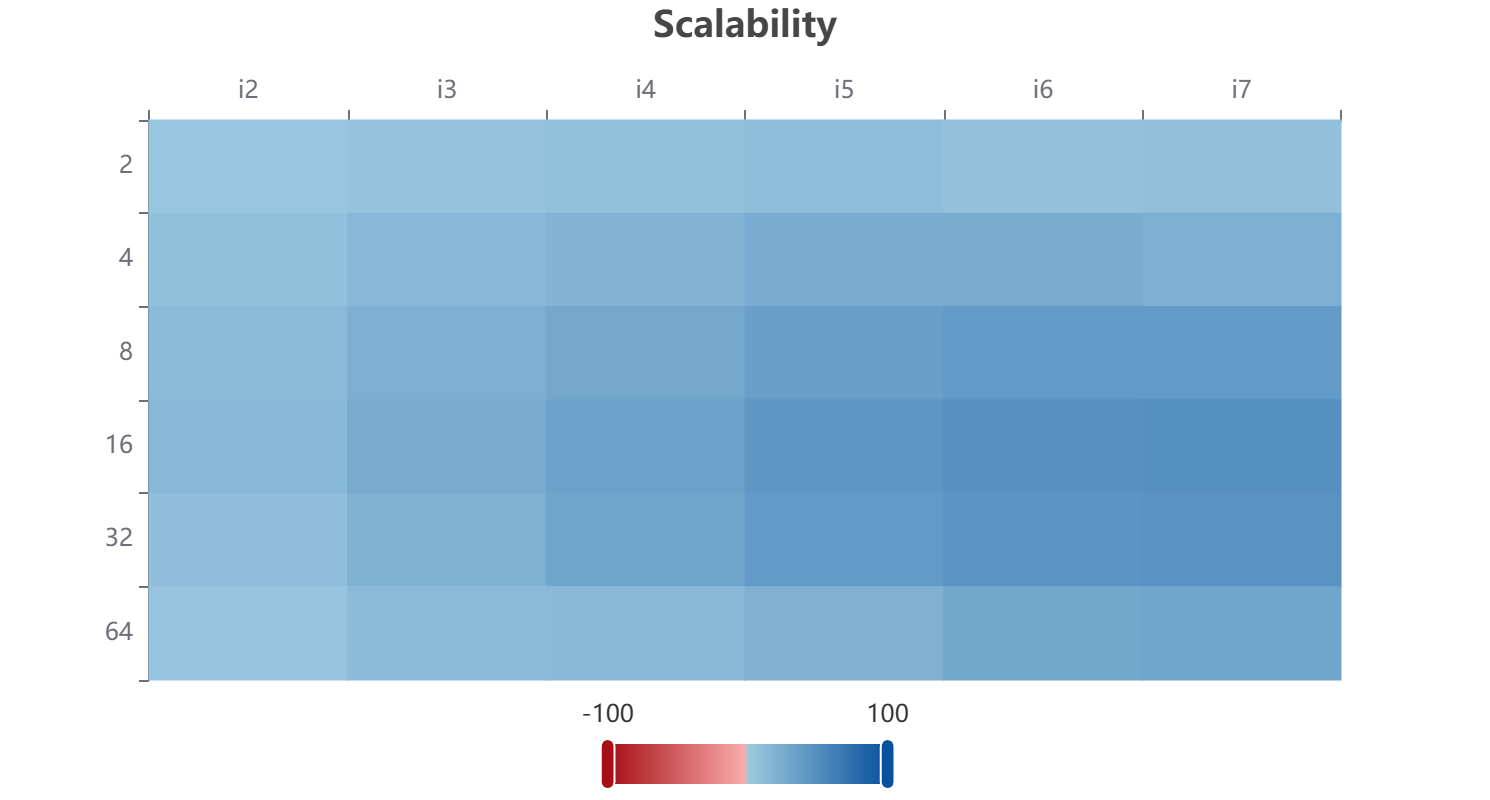
\includegraphics[width=\textwidth]{images/v4_numa_spread_threads_Scalability_Whole_Program_(Region_0).png}
\caption{\texttt{spread} com lugares por CPU lógica.}
\end{subfigure}
\caption{Escalabilidade geral do programa inteiro nas quatro configurações. As linhas indicam o número de threads e as colunas, cargas crescentes.}
\label{fig:afinidades}
\end{figure}

Sem binding, o mapa alterna regiões favoráveis e desfavoráveis nas cargas maiores. O sistema operacional pode migrar as threads nessa configuração, mas não houve medição de migrações que permita relacioná-las à irregularidade observada.

Com \texttt{close+cores}, as cargas menores aparecem em azul e a faixa favorável avança para cargas maiores quando $p$ cresce. A afinidade mantém as threads em lugares próximos, mas o mapa não permite determinar quanto essa proximidade contribuiu para o resultado.

Com \texttt{close+threads}, a região desfavorável aparece nas cargas maiores para valores intermediários de $p$ e desaparece em $p=64$. A diferença em relação a \texttt{close+cores} mostra que a escolha entre lugares por núcleo e por CPU lógica afetou o resultado. Não é possível isolar a contribuição do SMT.

\texttt{spread+threads} é a única configuração com todas as células em azul. Os tons mais intensos concentram-se nas cargas médias e grandes entre 8 e 32 threads, e o mapa permanece favorável em 64 threads. Essa configuração distribui as threads entre os lugares disponíveis e apresentou o padrão mais regular no indicador geral do Viewer.

\appendix
\clearpage
\section*{Anexo A: Código completo sem instrumentação do PaScal}
O programa abaixo mantém o cálculo, a inicialização, as verificações de entrada e alocação, os cronômetros OpenMP, os diagnósticos e a saída opcional em arquivo. Foram removidos apenas os trechos específicos da instrumentação do PaScal.

\lstinputlisting{v4_numa_anexo.c}

\end{document}
